\documentclass[aspectratio=169,
				xcolor=table]{beamer}

% Load general definitions
\usepackage[utf8]{inputenc}
%\usepackage[T1]{fontenc}
\usepackage[brazil]{babel}
\usepackage{amsmath}
\usepackage{amsfonts}
\usepackage{amssymb}
\usepackage{graphicx}
\usepackage{verbatim}
\usepackage{cancel}
\usepackage{askmaps}
\usepackage{tabularx}
\usepackage[table]{xcolor}
%\usepackage{tikz}
\usepackage{multirow}
\usepackage{mathtools}
\usepackage{color, colortbl}
\usepackage{etoolbox}
\usepackage{pbox}
\usepackage{changepage}
\usepackage{xpatch}
\usepackage{array}
\usepackage{marvosym}
\usepackage{tabu}
\usepackage{multicol}
\usepackage{listings}
\usepackage{underscore}
\usepackage{filecontents}
\usepackage[]{algorithm2e}
\usepackage{ragged2e}

\newcolumntype{P}[1]{>{\centering\arraybackslash}m{#1}}
\definecolor{Gray}{gray}{0.75}
\definecolor{Gray2}{gray}{0.85}

\definecolor{lightBlue}{HTML}{DAE8FC}
\definecolor{Blue}{RGB}{51, 51, 204}

%\useinnertheme[lily]{rounded}
\usetheme{UniEvangelica}
%\usetheme{Copenhagen}
%\usetheme{Berlin}
%\usecolortheme{dolphin}
\tolerance=1
\emergencystretch=\maxdimen
\hyphenpenalty=10000
\hbadness=10000

\setbeamertemplate{navigation symbols}{}%remove navigation symbols


\let\olditem=\item% 
\renewcommand{\item}{\olditem \justifying}%
\def\center{\trivlist \centering\item\relax}
\def\endcenter{\endtrivlist}

\setbeamertemplate{itemize/enumerate body begin}{\large}
\setbeamertemplate{itemize/enumerate subbody begin}{\large}

\setbeamertemplate{itemize item}{\raisebox{0.1ex}{$\blacktriangleright$}\hskip0.1em}
\setbeamertemplate{itemize subitem}{\raisebox{0.1ex}{$\blacktriangleright$}\hskip0.1em}

\newcommand{\greenarrow}{\textcolor{green}{\rotatebox[origin=c]{180}{\MVArrowDown}}}

\newcommand{\redarrow}{\textcolor{red}{\MVArrowDown}}

%\newcommand{\ftable}{
%	\begin{table}
%		\large
%		\centering
%		\rowcolors{1}{\ifnumless{\rownum}{2}{Blue}{lightBlue}}{}
%}

\newenvironment{eftable}{
	\begin{table}
		\large
		\centering
		\rowcolors{1}{}{Blue}
		\rowcolors{1}{\ifnumless{\rownum}{2}{Blue}{lightBlue}}{}
	}
	{
	\end{table}
}


%\setbeamertemplate{frametitle}
%{
%	%\vspace*{-2em}	
%	\insertframetitle
%
%	 %\textcolor{white}{\LARGE \insertframetitle}
%
%}

% Specific definitions
\institute[]{\uppercase{Engenharia de Software}}
\title[]{Sistemas Distribuídos}
\subtitle[]{\uppercase{Modelos de Sistemas}}
\author[]{Prof. M.e Alexandre Tannus}
\date{Anápolis - 2022.1}

%\AtBeginSection{\frame{\tableofcontents[currentsection]}}

\begin{document}
	\begin{frame}
		\titlepage		
	\end{frame}

	\begin{frame}
		\tableofcontents
	\end{frame}	

	\section{Introdução}

	\begin{frame}{Introdução}
		\begin{itemize}
			\item Modelos descritivos
			\begin{itemize}
				\item Fornecem informações sobre propriedades e problemas de projeto dos sistemas distribuídos
			\end{itemize}
			\vspace{1em}
			\item Tipos
			\begin{itemize}
				\item Físico
				\item Arquitetura
				\item Fundamentais
				\begin{itemize}
					\item Interação
					\item Falha
					\item Segurança
				\end{itemize}
			\end{itemize}
		\end{itemize}
	\end{frame}
	
	\begin{frame}{Introdução}
		\begin{itemize}
			\item Modelos físicos
			\begin{itemize}
				\item Tipos de computadores e equipamentos
			\end{itemize}
			\vspace{1em}
			\item Modelos de arquitetura
			\begin{itemize}
				\item Tarefas computacionais e de comunicação
			\end{itemize}
			\vspace{1em}
			\item Modelos fundamentais
			\begin{itemize}
				\item Descrevem problemas individuais
			\end{itemize}
		\end{itemize}	
	
	\end{frame}

	\section{Modelos Físicos}
	\begin{frame}{Modelos físicos}
		\begin{itemize}
			\item Básico
			\begin{itemize}
				\item Conjunto de computadores interconectados e prontos para a passagem de mensagem
			\end{itemize}
			\vspace{1em}
			\item Três gerações
			\begin{itemize}
				\item Primitivos
				\item Adaptados para Internet
				\item Contemporâneos
			\end{itemize}
		\end{itemize}
	\end{frame}
	
	\begin{frame}{Sistemas Primitivos}
		\begin{itemize}
			\item Rede local
			\vspace{1em}
			\item Conectividade limitada
			\vspace{1em}
			\item Pequena variedade de serviços
			\vspace{1em}
			\item Homogeneidade de sistema
		\end{itemize}
	\end{frame}
	
	\begin{frame}{Sistemas Adaptados para Internet}
		\begin{itemize}
			\item Exploração da estrutura da Internet
			\vspace{1em}
			\item Sistemas globais
			\vspace{1em}
			\item Alta heterogeneidade
			\begin{itemize}
				\item Redes
				\item Arquiteturas
				\item Sistemas Operacionais
				\item Linguagens de programação
			\end{itemize}
			\vspace{1em}
			\item Desenvolvimentos de padrões abertos e middlewares
		\end{itemize}
	\end{frame}
	
	\begin{frame}{Sistemas Contemporâneos}
		\begin{itemize}
			\item Computação móvel
			\vspace{1em}
			\item Computação ubíqua
			\vspace{1em}
			\item Nuvem
			\vspace{1em}
			\item \textit{Clusters}
		\end{itemize}
	\end{frame}
	
	\begin{frame}{}
	\begin{eftable}
		\begin{tabular}{|m{2.7cm}|m{2.3cm}|m{4.5cm}|m{3.5cm}|}
			\hline 
			\textcolor{white}{Sistemas Distribuídos} & 
			\textcolor{white}{Primitivos} & 
			\textcolor{white}{Adaptados para Internet} & 
			\textcolor{white}{Contemporâneos}
			 \\ 
			\hline 
			Escala & Pequenos & Grandes 
			 & Ultragrandes \\ 
			\hline 
			Heterogeneidade & Limitada & Significativa 
			 & Maiores dimensões introduzidas
			 \\ 
			\hline 
			Sistemas abertos & Não é prioridade & Prioridade significativa
			 & Grande desafio para a pesquisa
			 \\ 
			\hline 
			Qualidade de serviço & Em seu início
			 & Prioridade significativa, com introdução de vários serviços
			 & Grande desafio para a pesquisa
			 \\ 
			\hline 
		\end{tabular}
	\end{eftable}
	\end{frame}
	\section{Modelos de Arquitetura}	
	\begin{frame}{Modelos de Arquitetura}
		\begin{itemize}
			\item Arquitetura 
			\begin{itemize}
				\item Estrutura do sistema em termos de componentes especificados separadamente e suas inter-relações.
				\item Tem a função de garantir o bom funcionamento do sistema 
				\begin{itemize}
					\item Confianbilidade
					\item Escalabilidade
					\item Gerenciabilidade
					\item Adaptabilidade
					\item Rentabilidade
				\end{itemize}
			\end{itemize}
		\end{itemize}
	\end{frame}

	\begin{frame}{Modelos de Arquitetura}
		\begin{itemize}
			\item Cliente-servidor
			\vspace{1em}
			\item Peer-to-peer
			\vspace{1em}
			\item Objetos Distribuídos
			\vspace{1em}
			\item Componentes distribuídos
		\end{itemize}
	\end{frame}
	
	\begin{frame}{Elementos da arquitetura}
		\begin{itemize}
			\item Entidades de um sistema distribuído
			\begin{itemize}
				\item Quais são?
				\item Como se comunicam?
				\item Quais funções e responsabilidades possuem?
				\item Como são mapeadas na infraestrutura física?
			\end{itemize}
		\end{itemize}
	\end{frame}
	
	\begin{frame}{Quais são as entidades?}
		\begin{itemize}
			\item Visão do sistema
			\begin{itemize}
				\item Nós 
				\item Threads
			\end{itemize}

			\item Visão de programação
			\begin{itemize}
				\item Objetos
				\item Componentes 
				\item Serviços Web
			\end{itemize}
		\end{itemize}		
	\end{frame}
	
	\begin{frame}{Como se comunicam?}
		\begin{itemize}
			\item Comunicação entre processos
			\vspace{1em}
			\item Invocação remota
			\begin{itemize}
				\item Protocolos de requisição-resposta
				\item Chamada de Procedimento Remoto (RPC)
				\item Invocação de Método Remoto (RMI)
			\end{itemize}
		\end{itemize}
	\end{frame}
	
	\begin{frame}{Como se comunicam?}
		\begin{itemize}
			\item Comunicação indireta
			\begin{itemize}
				\item Comunicação em grupo
				\item Sistemas publicar-assinar
				\item Filas de mensagem
				\item Memória compartilhada distribuída
			\end{itemize}
		\end{itemize}
	\end{frame}
	
	\begin{frame}{Funções e responsabilidades}
		\begin{itemize}
			\item Processos assumem funções específicas para a realização de atividades 
			\vspace{1em}
			\item Estilos de arquitetura utilizadas
			\begin{itemize}
				\item Cliente-servidor
				\item Peer-to-peer
			\end{itemize}
		\end{itemize}
	\end{frame}
	
	\begin{frame}{Arquitetura cliente-servidor}
		\begin{itemize}
			\item Arquitetura mais utilizada
			\begin{figure}[hbtp]
			\centering
			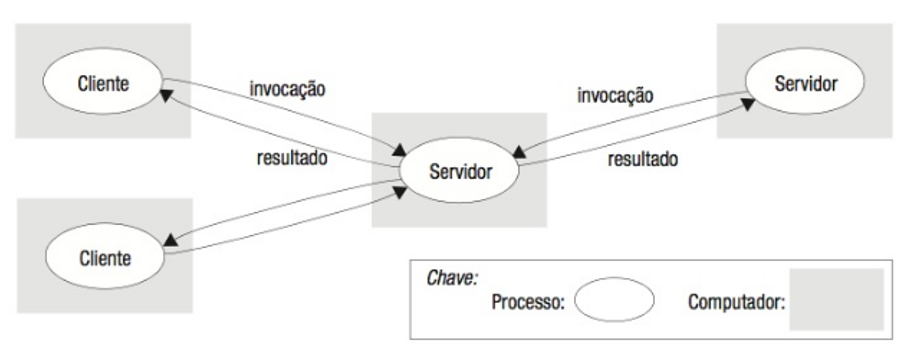
\includegraphics[height=5cm, keepaspectratio]{../figs/cap02/clienteservidor.png}
			\end{figure}			
		\end{itemize}
	\end{frame}
	
	\begin{frame}{Arquitetura peer-to-peer (P2P)}
		\begin{columns}
			\begin{column}{0.5\textwidth}
				\begin{itemize}
					\item Processos desempenham funções semelhantes
					\vspace{1em}
					\item Sistema descentralizado
					\vspace{1em}
					\item Mais complexo
				\end{itemize}
			\end{column}
			\begin{column}{0.5\textwidth}
				\begin{figure}[hbtp]
				\centering
				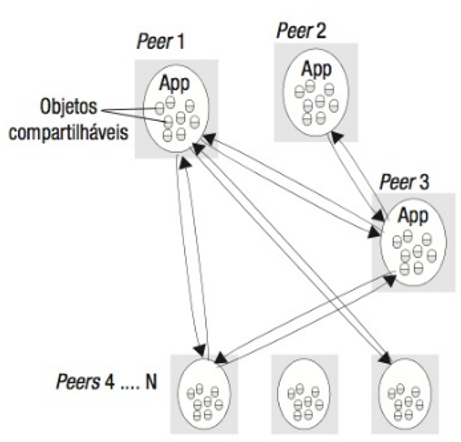
\includegraphics[width=0.8\textwidth, keepaspectratio]{../figs/cap02/p2p.png}
				\end{figure}	
			\end{column}
		\end{columns}
	\end{frame}
	
	\begin{frame}{Onde ficam fisicamente?}
		\begin{itemize}
			\item Localização de servidores e/ou clientes
			\begin{itemize}
				\item Segurança
				\item Confiabilidade
				\item Padrões de comunicação
				\item Carga de equipamentos presentes no sistema
				\item Qualidade da comunicação
			\end{itemize}
		\end{itemize}
	\end{frame}
	
	\begin{frame}{Padrões arquitetônicos}
		\begin{itemize}
			\item Combinações de elementos primitivos de arquitetura
			\vspace{1em}
			\item Tipos
			\begin{itemize}
				\item Camadas lógicas (\textit{layer})
				\item Camadas físicas (\textit{tier})
				\item Thin Clients
				\item Serviços Web
			\end{itemize}
		\end{itemize}
	\end{frame}
	
	\begin{frame}{Camadas lógicas}	
		\begin{figure}[hbtp]
		\centering
		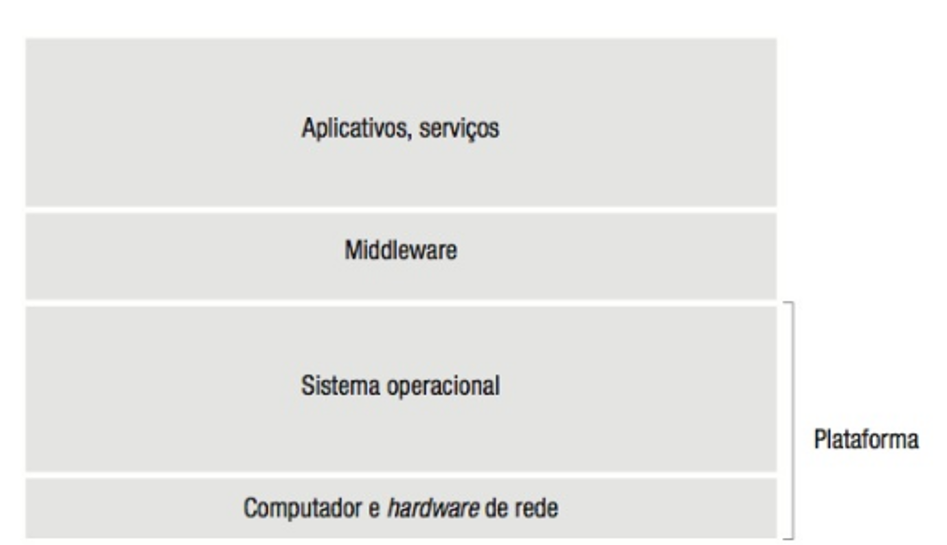
\includegraphics[width=0.8\textwidth, keepaspectratio]{../figs/cap02/camadafisica.png}
		\end{figure}	
	\end{frame}
	
	\begin{frame}{Camadas físicas}
		\begin{itemize}
			\item Complementar às camadas lógicas
			\vspace{1em}
			\item Funcionalidades de cada camada lógica
			\vspace{1em}
			\item Divisão em duas ou três camadas
		\end{itemize}
	\end{frame}
	
	\begin{frame}{Arquitetura de duas camadas}
		\begin{figure}[hbtp]
		\centering
		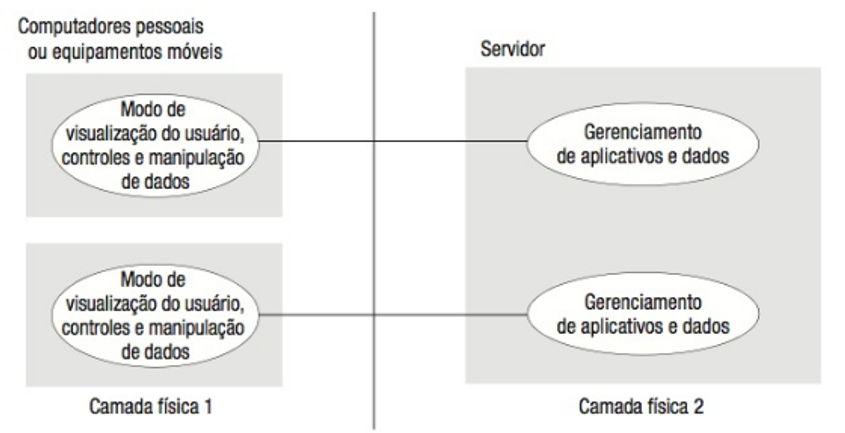
\includegraphics[width=0.9\textwidth, keepaspectratio]{../figs/cap02/duascamadas.png}
		\end{figure}
	\end{frame}
	
	\begin{frame}{Arquitetura de três camadas}
		\begin{figure}[hbtp]
		\centering
		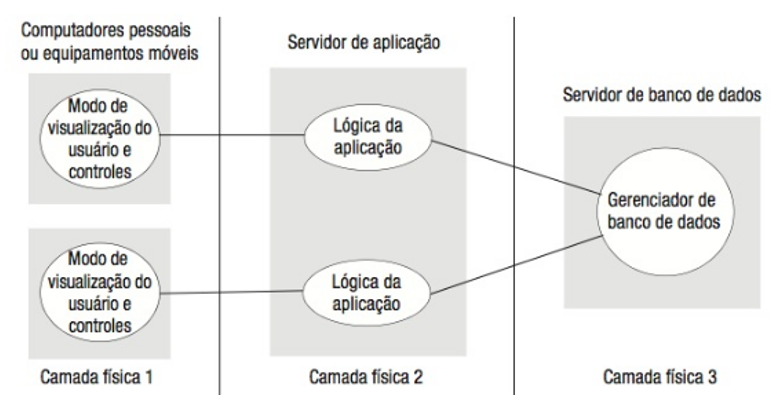
\includegraphics[width=0.9\textwidth, keepaspectratio]{../figs/cap02/trescamadas.png}
		\end{figure}
	\end{frame}

	\begin{frame}{Thin Clients}
		\begin{figure}[hbtp]
		\centering
		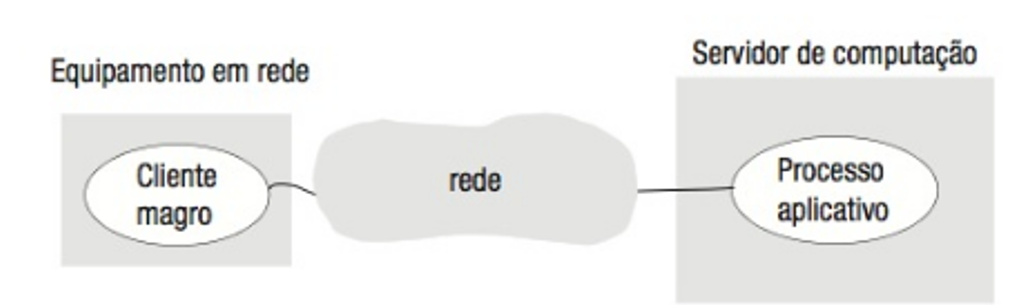
\includegraphics[width=0.9\textwidth, keepaspectratio]{../figs/cap02/thin.png}
		\end{figure}
	\end{frame}

	\begin{frame}{}
	\end{frame}	
\end{document}
